\documentclass[a4paper,12pt]{article}

	%\usepackage[latin1]{inputenc}
	\usepackage[portuguese]{babel}

    \usepackage[breakable]{tcolorbox}
    \usepackage{parskip} % Stop auto-indenting (to mimic markdown behaviour)
    \usepackage{textgreek}

    
    
    \usepackage{iftex}
    \ifPDFTeX
    	\usepackage[T1]{fontenc}
    	\usepackage{mathpazo}
    \else
    	\usepackage{fontspec}
    \fi

    % Basic figure setup, for now with no caption control since it's done
    % automatically by Pandoc (which extracts ![](path) syntax from Markdown).
    \usepackage{graphicx}
    % Maintain compatibility with old templates. Remove in nbconvert 6.0
    \let\Oldincludegraphics\includegraphics
    % Ensure that by default, figures have no caption (until we provide a
    % proper Figure object with a Caption API and a way to capture that
    % in the conversion process - todo).
    \usepackage[justification=centering]{caption}
    %\DeclareCaptionFormat{nocaption}{}
    \captionsetup{aboveskip=0pt,belowskip=0pt}

    \usepackage{float}
    \floatplacement{figure}{H} % forces figures to be placed at the correct location
    \floatplacement{table}{H} % forces tables to be placed at the correct location
    \usepackage{xcolor} % Allow colors to be defined
    \usepackage{enumerate} % Needed for markdown enumerations to work
    \usepackage{geometry} % Used to adjust the document margins
    \usepackage{amsmath} % Equations
    \usepackage{amssymb} % Equations
    \usepackage{textcomp} % defines textquotesingle
    % Hack from http://tex.stackexchange.com/a/47451/13684:
    \AtBeginDocument{%
        \def\PYZsq{\textquotesingle}% Upright quotes in Pygmentized code
    }
    \usepackage{upquote} % Upright quotes for verbatim code
    \usepackage{eurosym} % defines \euro
    \usepackage[mathletters]{ucs} % Extended unicode (utf-8) support
    \usepackage{fancyvrb} % verbatim replacement that allows latex
    \usepackage{grffile} % extends the file name processing of package graphics 
                         % to support a larger range
    \makeatletter % fix for old versions of grffile with XeLaTeX
    \@ifpackagelater{grffile}{2019/11/01}
    {
      % Do nothing on new versions
    }
    {
      \def\Gread@@xetex#1{%
        \IfFileExists{"\Gin@base".bb}%
        {\Gread@eps{\Gin@base.bb}}%
        {\Gread@@xetex@aux#1}%
      }
    }
    \makeatother
    \usepackage[Export]{adjustbox} % Used to constrain images to a maximum size
    \adjustboxset{max size={0.9\linewidth}{0.9\paperheight}}

    % The hyperref package gives us a pdf with properly built
    % internal navigation ('pdf bookmarks' for the table of contents,
    % internal cross-reference links, web links for URLs, etc.)
    \usepackage{hyperref}
    % The default LaTeX title has an obnoxious amount of whitespace. By default,
    % titling removes some of it. It also provides customization options.
    \usepackage{titling}
    \usepackage{longtable} % longtable support required by pandoc >1.10
    \usepackage{booktabs}  % table support for pandoc > 1.12.2
    \usepackage[inline]{enumitem} % IRkernel/repr support (it uses the enumerate* environment)
    \usepackage[normalem]{ulem} % ulem is needed to support strikethroughs (\sout)
                                % normalem makes italics be italics, not underlines
    \usepackage{mathrsfs}
    

    
    % Colors for the hyperref package
    \definecolor{urlcolor}{rgb}{0,0,0} %{0,0,0.5} é azul escuro
    \definecolor{linkcolor}{rgb}{0,0,0}
    \definecolor{citecolor}{rgb}{0,0,0}

    % ANSI colors
    \definecolor{ansi-black}{HTML}{3E424D}
    \definecolor{ansi-black-intense}{HTML}{282C36}
    \definecolor{ansi-red}{HTML}{E75C58}
    \definecolor{ansi-red-intense}{HTML}{B22B31}
    \definecolor{ansi-green}{HTML}{00A250}
    \definecolor{ansi-green-intense}{HTML}{007427}
    \definecolor{ansi-yellow}{HTML}{DDB62B}
    \definecolor{ansi-yellow-intense}{HTML}{B27D12}
    \definecolor{ansi-blue}{HTML}{208FFB}
    \definecolor{ansi-blue-intense}{HTML}{0065CA}
    \definecolor{ansi-magenta}{HTML}{D160C4}
    \definecolor{ansi-magenta-intense}{HTML}{A03196}
    \definecolor{ansi-cyan}{HTML}{60C6C8}
    \definecolor{ansi-cyan-intense}{HTML}{258F8F}
    \definecolor{ansi-white}{HTML}{C5C1B4}
    \definecolor{ansi-white-intense}{HTML}{A1A6B2}
    \definecolor{ansi-default-inverse-fg}{HTML}{FFFFFF}
    \definecolor{ansi-default-inverse-bg}{HTML}{000000}

    % common color for the border for error outputs.
    \definecolor{outerrorbackground}{HTML}{FFDFDF}

    % commands and environments needed by pandoc snippets
    % extracted from the output of `pandoc -s`
    \providecommand{\tightlist}{%
      \setlength{\itemsep}{0pt}\setlength{\parskip}{0pt}}
    \DefineVerbatimEnvironment{Highlighting}{Verbatim}{commandchars=\\\{\}}
    % Add ',fontsize=\small' for more characters per line
    \newenvironment{Shaded}{}{}
    \newcommand{\KeywordTok}[1]{\textcolor[rgb]{0.00,0.44,0.13}{\textbf{{#1}}}}
    \newcommand{\DataTypeTok}[1]{\textcolor[rgb]{0.56,0.13,0.00}{{#1}}}
    \newcommand{\DecValTok}[1]{\textcolor[rgb]{0.25,0.63,0.44}{{#1}}}
    \newcommand{\BaseNTok}[1]{\textcolor[rgb]{0.25,0.63,0.44}{{#1}}}
    \newcommand{\FloatTok}[1]{\textcolor[rgb]{0.25,0.63,0.44}{{#1}}}
    \newcommand{\CharTok}[1]{\textcolor[rgb]{0.25,0.44,0.63}{{#1}}}
    \newcommand{\StringTok}[1]{\textcolor[rgb]{0.25,0.44,0.63}{{#1}}}
    \newcommand{\CommentTok}[1]{\textcolor[rgb]{0.38,0.63,0.69}{\textit{{#1}}}}
    \newcommand{\OtherTok}[1]{\textcolor[rgb]{0.00,0.44,0.13}{{#1}}}
    \newcommand{\AlertTok}[1]{\textcolor[rgb]{1.00,0.00,0.00}{\textbf{{#1}}}}
    \newcommand{\FunctionTok}[1]{\textcolor[rgb]{0.02,0.16,0.49}{{#1}}}
    \newcommand{\RegionMarkerTok}[1]{{#1}}
    \newcommand{\ErrorTok}[1]{\textcolor[rgb]{1.00,0.00,0.00}{\textbf{{#1}}}}
    \newcommand{\NormalTok}[1]{{#1}}
    
    % Additional commands for more recent versions of Pandoc
    \newcommand{\ConstantTok}[1]{\textcolor[rgb]{0.53,0.00,0.00}{{#1}}}
    \newcommand{\SpecialCharTok}[1]{\textcolor[rgb]{0.25,0.44,0.63}{{#1}}}
    \newcommand{\VerbatimStringTok}[1]{\textcolor[rgb]{0.25,0.44,0.63}{{#1}}}
    \newcommand{\SpecialStringTok}[1]{\textcolor[rgb]{0.73,0.40,0.53}{{#1}}}
    \newcommand{\ImportTok}[1]{{#1}}
    \newcommand{\DocumentationTok}[1]{\textcolor[rgb]{0.73,0.13,0.13}{\textit{{#1}}}}
    \newcommand{\AnnotationTok}[1]{\textcolor[rgb]{0.38,0.63,0.69}{\textbf{\textit{{#1}}}}}
    \newcommand{\CommentVarTok}[1]{\textcolor[rgb]{0.38,0.63,0.69}{\textbf{\textit{{#1}}}}}
    \newcommand{\VariableTok}[1]{\textcolor[rgb]{0.10,0.09,0.49}{{#1}}}
    \newcommand{\ControlFlowTok}[1]{\textcolor[rgb]{0.00,0.44,0.13}{\textbf{{#1}}}}
    \newcommand{\OperatorTok}[1]{\textcolor[rgb]{0.40,0.40,0.40}{{#1}}}
    \newcommand{\BuiltInTok}[1]{{#1}}
    \newcommand{\ExtensionTok}[1]{{#1}}
    \newcommand{\PreprocessorTok}[1]{\textcolor[rgb]{0.74,0.48,0.00}{{#1}}}
    \newcommand{\AttributeTok}[1]{\textcolor[rgb]{0.49,0.56,0.16}{{#1}}}
    \newcommand{\InformationTok}[1]{\textcolor[rgb]{0.38,0.63,0.69}{\textbf{\textit{{#1}}}}}
    \newcommand{\WarningTok}[1]{\textcolor[rgb]{0.38,0.63,0.69}{\textbf{\textit{{#1}}}}}
    
    
    % Define a nice break command that doesn't care if a line doesn't already
    % exist.
    \def\br{\hspace*{\fill} \\* }
    % Math Jax compatibility definitions
    \def\gt{>}
    \def\lt{<}
    \let\Oldtex\TeX
    \let\Oldlatex\LaTeX
    \renewcommand{\TeX}{\textrm{\Oldtex}}
    \renewcommand{\LaTeX}{\textrm{\Oldlatex}}
   
    
    
    
    
    
% Pygments definitions
\makeatletter
\def\PY@reset{\let\PY@it=\relax \let\PY@bf=\relax%
    \let\PY@ul=\relax \let\PY@tc=\relax%
    \let\PY@bc=\relax \let\PY@ff=\relax}
\def\PY@tok#1{\csname PY@tok@#1\endcsname}
\def\PY@toks#1+{\ifx\relax#1\empty\else%
    \PY@tok{#1}\expandafter\PY@toks\fi}
\def\PY@do#1{\PY@bc{\PY@tc{\PY@ul{%
    \PY@it{\PY@bf{\PY@ff{#1}}}}}}}
\def\PY#1#2{\PY@reset\PY@toks#1+\relax+\PY@do{#2}}

\expandafter\def\csname PY@tok@w\endcsname{\def\PY@tc##1{\textcolor[rgb]{0.73,0.73,0.73}{##1}}}
\expandafter\def\csname PY@tok@c\endcsname{\let\PY@it=\textit\def\PY@tc##1{\textcolor[rgb]{0.25,0.50,0.50}{##1}}}
\expandafter\def\csname PY@tok@cp\endcsname{\def\PY@tc##1{\textcolor[rgb]{0.74,0.48,0.00}{##1}}}
\expandafter\def\csname PY@tok@k\endcsname{\let\PY@bf=\textbf\def\PY@tc##1{\textcolor[rgb]{0.00,0.50,0.00}{##1}}}
\expandafter\def\csname PY@tok@kp\endcsname{\def\PY@tc##1{\textcolor[rgb]{0.00,0.50,0.00}{##1}}}
\expandafter\def\csname PY@tok@kt\endcsname{\def\PY@tc##1{\textcolor[rgb]{0.69,0.00,0.25}{##1}}}
\expandafter\def\csname PY@tok@o\endcsname{\def\PY@tc##1{\textcolor[rgb]{0.40,0.40,0.40}{##1}}}
\expandafter\def\csname PY@tok@ow\endcsname{\let\PY@bf=\textbf\def\PY@tc##1{\textcolor[rgb]{0.67,0.13,1.00}{##1}}}
\expandafter\def\csname PY@tok@nb\endcsname{\def\PY@tc##1{\textcolor[rgb]{0.00,0.50,0.00}{##1}}}
\expandafter\def\csname PY@tok@nf\endcsname{\def\PY@tc##1{\textcolor[rgb]{0.00,0.00,1.00}{##1}}}
\expandafter\def\csname PY@tok@nc\endcsname{\let\PY@bf=\textbf\def\PY@tc##1{\textcolor[rgb]{0.00,0.00,1.00}{##1}}}
\expandafter\def\csname PY@tok@nn\endcsname{\let\PY@bf=\textbf\def\PY@tc##1{\textcolor[rgb]{0.00,0.00,1.00}{##1}}}
\expandafter\def\csname PY@tok@ne\endcsname{\let\PY@bf=\textbf\def\PY@tc##1{\textcolor[rgb]{0.82,0.25,0.23}{##1}}}
\expandafter\def\csname PY@tok@nv\endcsname{\def\PY@tc##1{\textcolor[rgb]{0.10,0.09,0.49}{##1}}}
\expandafter\def\csname PY@tok@no\endcsname{\def\PY@tc##1{\textcolor[rgb]{0.53,0.00,0.00}{##1}}}
\expandafter\def\csname PY@tok@nl\endcsname{\def\PY@tc##1{\textcolor[rgb]{0.63,0.63,0.00}{##1}}}
\expandafter\def\csname PY@tok@ni\endcsname{\let\PY@bf=\textbf\def\PY@tc##1{\textcolor[rgb]{0.60,0.60,0.60}{##1}}}
\expandafter\def\csname PY@tok@na\endcsname{\def\PY@tc##1{\textcolor[rgb]{0.49,0.56,0.16}{##1}}}
\expandafter\def\csname PY@tok@nt\endcsname{\let\PY@bf=\textbf\def\PY@tc##1{\textcolor[rgb]{0.00,0.50,0.00}{##1}}}
\expandafter\def\csname PY@tok@nd\endcsname{\def\PY@tc##1{\textcolor[rgb]{0.67,0.13,1.00}{##1}}}
\expandafter\def\csname PY@tok@s\endcsname{\def\PY@tc##1{\textcolor[rgb]{0.73,0.13,0.13}{##1}}}
\expandafter\def\csname PY@tok@sd\endcsname{\let\PY@it=\textit\def\PY@tc##1{\textcolor[rgb]{0.73,0.13,0.13}{##1}}}
\expandafter\def\csname PY@tok@si\endcsname{\let\PY@bf=\textbf\def\PY@tc##1{\textcolor[rgb]{0.73,0.40,0.53}{##1}}}
\expandafter\def\csname PY@tok@se\endcsname{\let\PY@bf=\textbf\def\PY@tc##1{\textcolor[rgb]{0.73,0.40,0.13}{##1}}}
\expandafter\def\csname PY@tok@sr\endcsname{\def\PY@tc##1{\textcolor[rgb]{0.73,0.40,0.53}{##1}}}
\expandafter\def\csname PY@tok@ss\endcsname{\def\PY@tc##1{\textcolor[rgb]{0.10,0.09,0.49}{##1}}}
\expandafter\def\csname PY@tok@sx\endcsname{\def\PY@tc##1{\textcolor[rgb]{0.00,0.50,0.00}{##1}}}
\expandafter\def\csname PY@tok@m\endcsname{\def\PY@tc##1{\textcolor[rgb]{0.40,0.40,0.40}{##1}}}
\expandafter\def\csname PY@tok@gh\endcsname{\let\PY@bf=\textbf\def\PY@tc##1{\textcolor[rgb]{0.00,0.00,0.50}{##1}}}
\expandafter\def\csname PY@tok@gu\endcsname{\let\PY@bf=\textbf\def\PY@tc##1{\textcolor[rgb]{0.50,0.00,0.50}{##1}}}
\expandafter\def\csname PY@tok@gd\endcsname{\def\PY@tc##1{\textcolor[rgb]{0.63,0.00,0.00}{##1}}}
\expandafter\def\csname PY@tok@gi\endcsname{\def\PY@tc##1{\textcolor[rgb]{0.00,0.63,0.00}{##1}}}
\expandafter\def\csname PY@tok@gr\endcsname{\def\PY@tc##1{\textcolor[rgb]{1.00,0.00,0.00}{##1}}}
\expandafter\def\csname PY@tok@ge\endcsname{\let\PY@it=\textit}
\expandafter\def\csname PY@tok@gs\endcsname{\let\PY@bf=\textbf}
\expandafter\def\csname PY@tok@gp\endcsname{\let\PY@bf=\textbf\def\PY@tc##1{\textcolor[rgb]{0.00,0.00,0.50}{##1}}}
\expandafter\def\csname PY@tok@go\endcsname{\def\PY@tc##1{\textcolor[rgb]{0.53,0.53,0.53}{##1}}}
\expandafter\def\csname PY@tok@gt\endcsname{\def\PY@tc##1{\textcolor[rgb]{0.00,0.27,0.87}{##1}}}
\expandafter\def\csname PY@tok@err\endcsname{\def\PY@bc##1{\setlength{\fboxsep}{0pt}\fcolorbox[rgb]{1.00,0.00,0.00}{1,1,1}{\strut ##1}}}
\expandafter\def\csname PY@tok@kc\endcsname{\let\PY@bf=\textbf\def\PY@tc##1{\textcolor[rgb]{0.00,0.50,0.00}{##1}}}
\expandafter\def\csname PY@tok@kd\endcsname{\let\PY@bf=\textbf\def\PY@tc##1{\textcolor[rgb]{0.00,0.50,0.00}{##1}}}
\expandafter\def\csname PY@tok@kn\endcsname{\let\PY@bf=\textbf\def\PY@tc##1{\textcolor[rgb]{0.00,0.50,0.00}{##1}}}
\expandafter\def\csname PY@tok@kr\endcsname{\let\PY@bf=\textbf\def\PY@tc##1{\textcolor[rgb]{0.00,0.50,0.00}{##1}}}
\expandafter\def\csname PY@tok@bp\endcsname{\def\PY@tc##1{\textcolor[rgb]{0.00,0.50,0.00}{##1}}}
\expandafter\def\csname PY@tok@fm\endcsname{\def\PY@tc##1{\textcolor[rgb]{0.00,0.00,1.00}{##1}}}
\expandafter\def\csname PY@tok@vc\endcsname{\def\PY@tc##1{\textcolor[rgb]{0.10,0.09,0.49}{##1}}}
\expandafter\def\csname PY@tok@vg\endcsname{\def\PY@tc##1{\textcolor[rgb]{0.10,0.09,0.49}{##1}}}
\expandafter\def\csname PY@tok@vi\endcsname{\def\PY@tc##1{\textcolor[rgb]{0.10,0.09,0.49}{##1}}}
\expandafter\def\csname PY@tok@vm\endcsname{\def\PY@tc##1{\textcolor[rgb]{0.10,0.09,0.49}{##1}}}
\expandafter\def\csname PY@tok@sa\endcsname{\def\PY@tc##1{\textcolor[rgb]{0.73,0.13,0.13}{##1}}}
\expandafter\def\csname PY@tok@sb\endcsname{\def\PY@tc##1{\textcolor[rgb]{0.73,0.13,0.13}{##1}}}
\expandafter\def\csname PY@tok@sc\endcsname{\def\PY@tc##1{\textcolor[rgb]{0.73,0.13,0.13}{##1}}}
\expandafter\def\csname PY@tok@dl\endcsname{\def\PY@tc##1{\textcolor[rgb]{0.73,0.13,0.13}{##1}}}
\expandafter\def\csname PY@tok@s2\endcsname{\def\PY@tc##1{\textcolor[rgb]{0.73,0.13,0.13}{##1}}}
\expandafter\def\csname PY@tok@sh\endcsname{\def\PY@tc##1{\textcolor[rgb]{0.73,0.13,0.13}{##1}}}
\expandafter\def\csname PY@tok@s1\endcsname{\def\PY@tc##1{\textcolor[rgb]{0.73,0.13,0.13}{##1}}}
\expandafter\def\csname PY@tok@mb\endcsname{\def\PY@tc##1{\textcolor[rgb]{0.40,0.40,0.40}{##1}}}
\expandafter\def\csname PY@tok@mf\endcsname{\def\PY@tc##1{\textcolor[rgb]{0.40,0.40,0.40}{##1}}}
\expandafter\def\csname PY@tok@mh\endcsname{\def\PY@tc##1{\textcolor[rgb]{0.40,0.40,0.40}{##1}}}
\expandafter\def\csname PY@tok@mi\endcsname{\def\PY@tc##1{\textcolor[rgb]{0.40,0.40,0.40}{##1}}}
\expandafter\def\csname PY@tok@il\endcsname{\def\PY@tc##1{\textcolor[rgb]{0.40,0.40,0.40}{##1}}}
\expandafter\def\csname PY@tok@mo\endcsname{\def\PY@tc##1{\textcolor[rgb]{0.40,0.40,0.40}{##1}}}
\expandafter\def\csname PY@tok@ch\endcsname{\let\PY@it=\textit\def\PY@tc##1{\textcolor[rgb]{0.25,0.50,0.50}{##1}}}
\expandafter\def\csname PY@tok@cm\endcsname{\let\PY@it=\textit\def\PY@tc##1{\textcolor[rgb]{0.25,0.50,0.50}{##1}}}
\expandafter\def\csname PY@tok@cpf\endcsname{\let\PY@it=\textit\def\PY@tc##1{\textcolor[rgb]{0.25,0.50,0.50}{##1}}}
\expandafter\def\csname PY@tok@c1\endcsname{\let\PY@it=\textit\def\PY@tc##1{\textcolor[rgb]{0.25,0.50,0.50}{##1}}}
\expandafter\def\csname PY@tok@cs\endcsname{\let\PY@it=\textit\def\PY@tc##1{\textcolor[rgb]{0.25,0.50,0.50}{##1}}}

\def\PYZbs{\char`\\}
\def\PYZus{\char`\_}
\def\PYZob{\char`\{}
\def\PYZcb{\char`\}}
\def\PYZca{\char`\^}
\def\PYZam{\char`\&}
\def\PYZlt{\char`\<}
\def\PYZgt{\char`\>}
\def\PYZsh{\char`\#}
\def\PYZpc{\char`\%}
\def\PYZdl{\char`\$}
\def\PYZhy{\char`\-}
\def\PYZsq{\char`\'}
\def\PYZdq{\char`\"}
\def\PYZti{\char`\~}
% for compatibility with earlier versions
\def\PYZat{@}
\def\PYZlb{[}
\def\PYZrb{]}
\makeatother


    % For linebreaks inside Verbatim environment from package fancyvrb. 
    \makeatletter
        \newbox\Wrappedcontinuationbox 
        \newbox\Wrappedvisiblespacebox 
        \newcommand*\Wrappedvisiblespace {\textcolor{red}{\textvisiblespace}} 
        \newcommand*\Wrappedcontinuationsymbol {\textcolor{red}{\llap{\tiny$\m@th\hookrightarrow$}}} 
        \newcommand*\Wrappedcontinuationindent {3ex } 
        \newcommand*\Wrappedafterbreak {\kern\Wrappedcontinuationindent\copy\Wrappedcontinuationbox} 
        % Take advantage of the already applied Pygments mark-up to insert 
        % potential linebreaks for TeX processing. 
        %        {, <, #, %, $, ' and ": go to next line. 
        %        _, }, ^, &, >, - and ~: stay at end of broken line. 
        % Use of \textquotesingle for straight quote. 
        \newcommand*\Wrappedbreaksatspecials {% 
            \def\PYGZus{\discretionary{\char`\_}{\Wrappedafterbreak}{\char`\_}}% 
            \def\PYGZob{\discretionary{}{\Wrappedafterbreak\char`\{}{\char`\{}}% 
            \def\PYGZcb{\discretionary{\char`\}}{\Wrappedafterbreak}{\char`\}}}% 
            \def\PYGZca{\discretionary{\char`\^}{\Wrappedafterbreak}{\char`\^}}% 
            \def\PYGZam{\discretionary{\char`\&}{\Wrappedafterbreak}{\char`\&}}% 
            \def\PYGZlt{\discretionary{}{\Wrappedafterbreak\char`\<}{\char`\<}}% 
            \def\PYGZgt{\discretionary{\char`\>}{\Wrappedafterbreak}{\char`\>}}% 
            \def\PYGZsh{\discretionary{}{\Wrappedafterbreak\char`\#}{\char`\#}}% 
            \def\PYGZpc{\discretionary{}{\Wrappedafterbreak\char`\%}{\char`\%}}% 
            \def\PYGZdl{\discretionary{}{\Wrappedafterbreak\char`\$}{\char`\$}}% 
            \def\PYGZhy{\discretionary{\char`\-}{\Wrappedafterbreak}{\char`\-}}% 
            \def\PYGZsq{\discretionary{}{\Wrappedafterbreak\textquotesingle}{\textquotesingle}}% 
            \def\PYGZdq{\discretionary{}{\Wrappedafterbreak\char`\"}{\char`\"}}% 
            \def\PYGZti{\discretionary{\char`\~}{\Wrappedafterbreak}{\char`\~}}% 
        } 
        % Some characters . , ; ? ! / are not pygmentized. 
        % This macro makes them "active" and they will insert potential linebreaks 
        \newcommand*\Wrappedbreaksatpunct {% 
            \lccode`\~`\.\lowercase{\def~}{\discretionary{\hbox{\char`\.}}{\Wrappedafterbreak}{\hbox{\char`\.}}}% 
            \lccode`\~`\,\lowercase{\def~}{\discretionary{\hbox{\char`\,}}{\Wrappedafterbreak}{\hbox{\char`\,}}}% 
            \lccode`\~`\;\lowercase{\def~}{\discretionary{\hbox{\char`\;}}{\Wrappedafterbreak}{\hbox{\char`\;}}}% 
            \lccode`\~`\:\lowercase{\def~}{\discretionary{\hbox{\char`\:}}{\Wrappedafterbreak}{\hbox{\char`\:}}}% 
            \lccode`\~`\?\lowercase{\def~}{\discretionary{\hbox{\char`\?}}{\Wrappedafterbreak}{\hbox{\char`\?}}}% 
            \lccode`\~`\!\lowercase{\def~}{\discretionary{\hbox{\char`\!}}{\Wrappedafterbreak}{\hbox{\char`\!}}}% 
            \lccode`\~`\/\lowercase{\def~}{\discretionary{\hbox{\char`\/}}{\Wrappedafterbreak}{\hbox{\char`\/}}}% 
            \catcode`\.\active
            \catcode`\,\active 
            \catcode`\;\active
            \catcode`\:\active
            \catcode`\?\active
            \catcode`\!\active
            \catcode`\/\active 
            \lccode`\~`\~ 	
        }
    \makeatother

    \let\OriginalVerbatim=\Verbatim
    \makeatletter
    \renewcommand{\Verbatim}[1][1]{%
    	
    	%\fontfamily{fi4}
  		%\fontsize{11}{2}
  		\linespread{0.9}	
    	
        %\parskip\z@skip
        \sbox\Wrappedcontinuationbox {\Wrappedcontinuationsymbol}%
        \sbox\Wrappedvisiblespacebox {\FV@SetupFont\Wrappedvisiblespace}%
        \def\FancyVerbFormatLine ##1{\hsize\linewidth
            \vtop{\raggedright\hyphenpenalty\z@\exhyphenpenalty\z@
                \doublehyphendemerits\z@\finalhyphendemerits\z@
                \strut ##1\strut}%
        }%
        % If the linebreak is at a space, the latter will be displayed as visible
        % space at end of first line, and a continuation symbol starts next line.
        % Stretch/shrink are however usually zero for typewriter font.
        \def\FV@Space {%
            \nobreak\hskip\z@ plus\fontdimen3\font minus\fontdimen4\font
            \discretionary{\copy\Wrappedvisiblespacebox}{\Wrappedafterbreak}
            {\kern\fontdimen2\font}%
        }%
        
        % Allow breaks at special characters using \PYG... macros.
        \Wrappedbreaksatspecials
        % Breaks at punctuation characters . , ; ? ! and / need catcode=\active 	
        \OriginalVerbatim[#1,codes*=\Wrappedbreaksatpunct]%
    }
    \makeatother

    % Exact colors from NB
    \definecolor{incolor}{HTML}{303F9F}
    \definecolor{outcolor}{HTML}{D84315}
    \definecolor{cellborder}{HTML}{CFCFCF}
    \definecolor{cellbackground}{HTML}{F7F7F7}
    
    % prompt
    \makeatletter
    \newcommand{\boxspacing}{\kern\kvtcb@left@rule\kern\kvtcb@boxsep}
    \makeatother
    \newcommand{\prompt}[4]{ }
    

    
    % Prevent overflowing lines due to hard-to-break entities
    \sloppy 
    % Setup hyperref package
    \hypersetup{
      breaklinks=true,  % so long urls are correctly broken across lines
      colorlinks=true,
      urlcolor=urlcolor,
      linkcolor=linkcolor,
      citecolor=citecolor,
      }
    % Slightly bigger margins than the latex defaults
    
    \geometry{verbose,tmargin=1in,bmargin=1in,lmargin=1in,rmargin=1in}

 \linespread{1.25}
    
 
 \makeatletter
 
 \newcommand{\subtitle}[1]{\def\@subtitle{#1}}
 
 \renewcommand\maketitle{%
 		\begin{center}
 			{\large Universidade Federal do Rio Grande do Sul}\\
 			{\normalsize Escola de Engenharia}\\
 			{\normalsize Programa de Pós-Graduação em Engenharia Civil}\\[48pt] 
 			{\Large \@title }\\[8pt] 
 			{\large \@subtitle }\\[24pt] 
 		\end{center}
 		\begin{flushright}
 			{\normalsize \@author}\\[24pt] 
 		\end{flushright}
 		\begin{center}
 			{\@date}\\[0pt] 
 		\end{center}
 		\noindent\rule{17cm}{0.8pt}
 }
\makeatother

\author{Eduardo Pagnussat Titello}
\title{PEC00144 - Métodos Experimentais em Engenharia Civil}
\subtitle{Trabalho 2}
\date{Novembro de 2020}


\begin{document}

\maketitle


Este trabalho tem por objetivo: no tema de interesse, adotar um problema
imaginário de formulação explícita, com 2 ou mais parâmetros
dimensionais. Desenhar, formular e definir uma nova escala para o
problema, fazendo uma análise de mudança de escala de forma a poder
construir tal modelo.

    \begin{tcolorbox}[breakable, size=fbox, boxrule=1pt, pad at break*=1mm,colback=cellbackground, colframe=cellborder]
\prompt{In}{incolor}{1}{\boxspacing}
\begin{Verbatim}[commandchars=\\\{\}]
\PY{c+c1}{\PYZsh{} Importando e configurando módulos}
\PY{k+kn}{import} \PY{n+nn}{numpy} \PY{k}{as} \PY{n+nn}{np}
\PY{k+kn}{import} \PY{n+nn}{pandas} \PY{k}{as} \PY{n+nn}{pd} 
\PY{k+kn}{import} \PY{n+nn}{matplotlib}\PY{n+nn}{.}\PY{n+nn}{pyplot} \PY{k}{as} \PY{n+nn}{plt}
\PY{c+c1}{\PYZsh{}import matplotlib}
\PY{o}{\PYZpc{}}\PY{k}{config} InlineBackend.figure\PYZus{}format = \PYZsq{}svg\PYZsq{} \PYZsh{} Muda backend do jupyter para SVG ;)
\PY{k+kn}{import} \PY{n+nn}{jupyter2latex} \PY{k}{as} \PY{n+nn}{j2l} \PY{c+c1}{\PYZsh{} Uma maneira que encontrei para tabelas ficarem ok (github.com/dutitello/Jupyter2Latex)}
\PY{k+kn}{from} \PY{n+nn}{math} \PY{k+kn}{import} \PY{n}{pi}
\end{Verbatim}
\end{tcolorbox}

    \hypertarget{apresentauxe7uxe3o-do-problema}{%
\section{Apresentação do
problema}\label{apresentauxe7uxe3o-do-problema}}

O problema adotado consiste na avaliação das duas primeiras frequências
naturais de vibração de um poste em concreto armado, considerando seu
comportamento como elástico linear. O poste adotado tem comprimento
efetivo \(L= 12m\), seção constante de diâmetro externo \(d_e = 50cm\) e
espessura \(e=6 cm\), resultando em um diâmetro interno \(d_i = 38cm\),
conforme a figura:

\begin{figure}
\centering
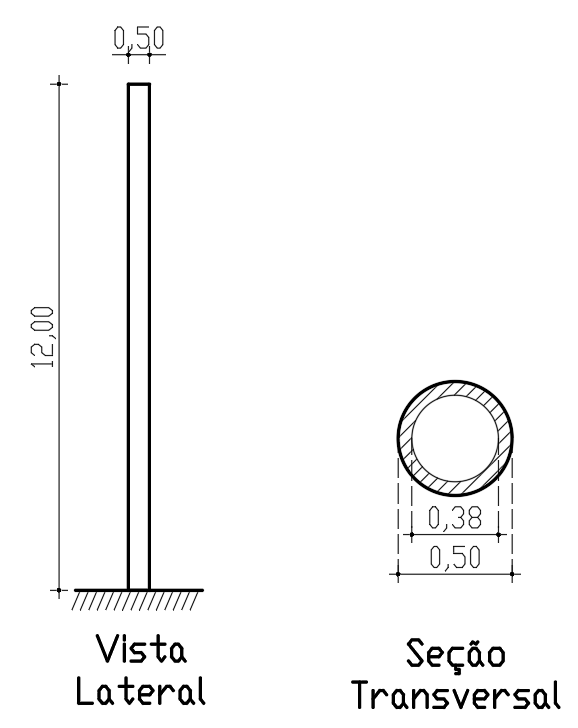
\includegraphics[scale=0.5]{Poste.png}
\caption{Poste}
\end{figure}

    Conforme Rocha (2020a), as frequências naturais de vibração de uma viga
engastada livre (modelo adotado para o poste) podem ser obtidas por
\ref{eq:wn}:

\begin{equation}
f_n = \frac{1}{2\pi} {\Big( \frac{\alpha_n}{L} \Big)}^2 \sqrt{\frac{EI}{\mu_L}}
\label{eq:wn}
\end{equation}

onde, para as duas primeiras frequências naturais, \(\alpha_1=1.88\) e
\(\alpha_2=4.69\), respectivamente, e \(\mu_L\) é a massa linear da
estrutura (massa/comprimento).

A área da seção transversal circular vazada \(A\) e seu momento de
inércia \(I\) são dados por:

\begin{equation}
A = \frac{\pi}{4}\big(d_e^2 - d_i^2 \big)
\label{eq:Ac}
\end{equation}

\begin{equation}
I = \frac{\pi}{64}\big(d_e^4 - d_i^4 \big)
\label{eq:Ic}
\end{equation}

    Adotando o subíndice ``\(_c\)'' para representar a estrutura real em
concreto, sendo empregado concreto da classe C25, o módulo de
elasticidade do material é \(E_c=28 GPa\), enquanto sua densidade é
aproximadamente \(\rho_c=2500 kg/m^3\). As propriedades da estrutura
original são então:

    \begin{tcolorbox}[breakable, size=fbox, boxrule=1pt, pad at break*=1mm,colback=cellbackground, colframe=cellborder]
\prompt{In}{incolor}{2}{\boxspacing}
\begin{Verbatim}[commandchars=\\\{\}]
\PY{n}{L\PYZus{}c}   \PY{o}{=} \PY{l+m+mf}{12.0}   \PY{c+c1}{\PYZsh{} m}
\PY{n}{de\PYZus{}c}  \PY{o}{=} \PY{l+m+mf}{0.50}   \PY{c+c1}{\PYZsh{} m}
\PY{n}{di\PYZus{}c}  \PY{o}{=} \PY{l+m+mf}{0.38}   \PY{c+c1}{\PYZsh{} m}
\PY{n}{E\PYZus{}c}   \PY{o}{=} \PY{l+m+mf}{28.0E9} \PY{c+c1}{\PYZsh{} N/m\PYZca{}2}
\PY{n}{rho\PYZus{}c} \PY{o}{=} \PY{l+m+mi}{2500}   \PY{c+c1}{\PYZsh{} kg/m\PYZca{}3}

\PY{n}{A\PYZus{}c}   \PY{o}{=} \PY{n}{pi}\PY{o}{/}\PY{l+m+mi}{4}\PY{o}{*}\PY{p}{(}\PY{n}{de\PYZus{}c}\PY{o}{*}\PY{o}{*}\PY{l+m+mi}{2} \PY{o}{\PYZhy{}} \PY{n}{di\PYZus{}c}\PY{o}{*}\PY{o}{*}\PY{l+m+mi}{2}\PY{p}{)}  \PY{c+c1}{\PYZsh{} m\PYZca{}2}
\PY{n}{I\PYZus{}c}   \PY{o}{=} \PY{n}{pi}\PY{o}{/}\PY{l+m+mi}{64}\PY{o}{*}\PY{p}{(}\PY{n}{de\PYZus{}c}\PY{o}{*}\PY{o}{*}\PY{l+m+mi}{4} \PY{o}{\PYZhy{}} \PY{n}{di\PYZus{}c}\PY{o}{*}\PY{o}{*}\PY{l+m+mi}{4}\PY{p}{)} \PY{c+c1}{\PYZsh{} m\PYZca{}4}

\PY{n}{EI\PYZus{}c}  \PY{o}{=} \PY{n}{E\PYZus{}c}\PY{o}{*}\PY{n}{I\PYZus{}c}   \PY{c+c1}{\PYZsh{} Nm\PYZca{}2}
\PY{n}{muL\PYZus{}c} \PY{o}{=} \PY{n}{A\PYZus{}c}\PY{o}{*}\PY{n}{rho\PYZus{}c} \PY{c+c1}{\PYZsh{} kg/m}
\PY{n}{m\PYZus{}c}   \PY{o}{=} \PY{n}{muL\PYZus{}c}\PY{o}{*}\PY{n}{L\PYZus{}c} \PY{c+c1}{\PYZsh{} kg}

\PY{n+nb}{print}\PY{p}{(}\PY{l+s+sa}{f}\PY{l+s+s1}{\PYZsq{}\PYZsq{}\PYZsq{}}
\PY{l+s+s1}{Propriedades da estrutura:}
\PY{l+s+s1}{    Área da seção             A\PYZus{}c = }\PY{l+s+si}{\PYZob{}}\PY{n}{A\PYZus{}c}\PY{l+s+si}{:}\PY{l+s+s1}{.3f}\PY{l+s+si}{\PYZcb{}}\PY{l+s+s1}{ m\PYZca{}2}
\PY{l+s+s1}{    Momento de Inércia        I\PYZus{}c = }\PY{l+s+si}{\PYZob{}}\PY{n}{I\PYZus{}c}\PY{l+s+si}{:}\PY{l+s+s1}{.3E}\PY{l+s+si}{\PYZcb{}}\PY{l+s+s1}{ m\PYZca{}4 }
\PY{l+s+s1}{    Rigidez EI             (EI)\PYZus{}c = }\PY{l+s+si}{\PYZob{}}\PY{n}{EI\PYZus{}c}\PY{l+s+si}{:}\PY{l+s+s1}{.3E}\PY{l+s+si}{\PYZcb{}}\PY{l+s+s1}{ N.m\PYZca{}2}
\PY{l+s+s1}{    Massa linear             μL\PYZus{}c = }\PY{l+s+si}{\PYZob{}}\PY{n}{muL\PYZus{}c}\PY{l+s+si}{:}\PY{l+s+s1}{.2f}\PY{l+s+si}{\PYZcb{}}\PY{l+s+s1}{ kg/m}
\PY{l+s+s1}{    Massa total               m\PYZus{}c = }\PY{l+s+si}{\PYZob{}}\PY{n}{m\PYZus{}c}\PY{l+s+si}{:}\PY{l+s+s1}{.2f}\PY{l+s+si}{\PYZcb{}}\PY{l+s+s1}{ kg}
\PY{l+s+s1}{\PYZsq{}\PYZsq{}\PYZsq{}}\PY{p}{)}
\end{Verbatim}
\end{tcolorbox}

    \begin{Verbatim}[commandchars=\\\{\}]

Propriedades da estrutura:
    Área da seção             A\_c = 0.083 m\^{}2
    Momento de Inércia        I\_c = 2.044E-03 m\^{}4
    Rigidez EI             (EI)\_c = 5.724E+07 N.m\^{}2
    Massa linear             μL\_c = 207.35 kg/m
    Massa total               m\_c = 2488.14 kg

    \end{Verbatim}

    \hypertarget{definiuxe7uxe3o-do-modelo-reduzido}{%
\section{Definição do modelo
reduzido}\label{definiuxe7uxe3o-do-modelo-reduzido}}

Conforme a expressão \ref{eq:wn}, as frequências naturais da estrutura
são dependentes do seu comprimento \(L\), da sua rigidez à flexão \(EI\)
e da sua massa linear \(\mu_L\). Em relação às dimensões, o fator de
escala adotado é 1:25. Adotando um modelo reduzido em alumínio, com
módulo de elasticidade \(E_m=70GPa\) e densidade \(\rho_m=2700kg/m^3\),
os demais fatores de escala adotados são relativos à rigidez \(EI\) e a
massa linear \(\mu_L\).

Os fatores de escala \(EI\) e \(\mu_L\) devem considerar perfis de
alumínio comercialmente viáveis, dessa forma, é adotado o perfil
cilindrico cheio VR-002 da Aluita (Aluita, 2019), de diâmetro externo
\(d_{e,m}=6.00mm\). O perfil cilíndrico cheio é adotado de forma a
reduzir as frequências naturais do modelo reduzido, visto que esse
possuí razão \(EI/\mu_L\) menor que os perfis tubulares da marca (TR-002
e TR-004). Os fatores de escala são então obtidos relacionando as
propriedades da seção do modelo à seção do poste:

    \begin{tcolorbox}[breakable, size=fbox, boxrule=1pt, pad at break*=1mm,colback=cellbackground, colframe=cellborder]
\prompt{In}{incolor}{3}{\boxspacing}
\begin{Verbatim}[commandchars=\\\{\}]
\PY{c+c1}{\PYZsh{} Perfil tubular TR\PYZhy{}004}
\PY{c+c1}{\PYZsh{}de\PYZus{}m  = 12.70/1000 \PYZsh{} m}
\PY{c+c1}{\PYZsh{}di\PYZus{}m  = 10.22/1000 \PYZsh{} m}
\PY{c+c1}{\PYZsh{} Perfil tubular TR\PYZhy{}002}
\PY{c+c1}{\PYZsh{}de\PYZus{}m  = 9.53/1000  \PYZsh{} m}
\PY{c+c1}{\PYZsh{}di\PYZus{}m  = 6.35/1000  \PYZsh{} m}
\PY{c+c1}{\PYZsh{} Perfil cilíndrico VR\PYZhy{}002}
\PY{n}{de\PYZus{}m}  \PY{o}{=} \PY{l+m+mi}{6}\PY{o}{/}\PY{l+m+mi}{1000}     \PY{c+c1}{\PYZsh{} m}
\PY{n}{di\PYZus{}m}  \PY{o}{=} \PY{l+m+mi}{0}\PY{o}{/}\PY{l+m+mi}{1000}     \PY{c+c1}{\PYZsh{} m}
\PY{n}{E\PYZus{}m}   \PY{o}{=} \PY{l+m+mf}{70.0E9}     \PY{c+c1}{\PYZsh{} N/m\PYZca{}2}
\PY{n}{rho\PYZus{}m} \PY{o}{=} \PY{l+m+mi}{2700}       \PY{c+c1}{\PYZsh{} kg/m\PYZca{}3}

\PY{n}{A\PYZus{}m}   \PY{o}{=} \PY{n}{pi}\PY{o}{/}\PY{l+m+mi}{4}\PY{o}{*}\PY{p}{(}\PY{n}{de\PYZus{}m}\PY{o}{*}\PY{o}{*}\PY{l+m+mi}{2} \PY{o}{\PYZhy{}} \PY{n}{di\PYZus{}m}\PY{o}{*}\PY{o}{*}\PY{l+m+mi}{2}\PY{p}{)}  \PY{c+c1}{\PYZsh{} m\PYZca{}2}
\PY{n}{I\PYZus{}m}   \PY{o}{=} \PY{n}{pi}\PY{o}{/}\PY{l+m+mi}{64}\PY{o}{*}\PY{p}{(}\PY{n}{de\PYZus{}m}\PY{o}{*}\PY{o}{*}\PY{l+m+mi}{4} \PY{o}{\PYZhy{}} \PY{n}{di\PYZus{}m}\PY{o}{*}\PY{o}{*}\PY{l+m+mi}{4}\PY{p}{)} \PY{c+c1}{\PYZsh{} m\PYZca{}4}
\PY{n}{EI\PYZus{}m}  \PY{o}{=} \PY{n}{E\PYZus{}m}\PY{o}{*}\PY{n}{I\PYZus{}m}    \PY{c+c1}{\PYZsh{} Nm\PYZca{}2}
\PY{n}{muL\PYZus{}m} \PY{o}{=} \PY{n}{A\PYZus{}m}\PY{o}{*}\PY{n}{rho\PYZus{}m}  \PY{c+c1}{\PYZsh{} kg/m}

\PY{n+nb}{print}\PY{p}{(}\PY{l+s+sa}{f}\PY{l+s+s1}{\PYZsq{}\PYZsq{}\PYZsq{}}
\PY{l+s+s1}{Propriedades do modelo reduzido:}
\PY{l+s+s1}{    Área da seção             A\PYZus{}m = }\PY{l+s+si}{\PYZob{}}\PY{n}{A\PYZus{}m}\PY{l+s+si}{:}\PY{l+s+s1}{.3E}\PY{l+s+si}{\PYZcb{}}\PY{l+s+s1}{ m\PYZca{}2}
\PY{l+s+s1}{    Momento de Inércia        I\PYZus{}m = }\PY{l+s+si}{\PYZob{}}\PY{n}{I\PYZus{}m}\PY{l+s+si}{:}\PY{l+s+s1}{.3E}\PY{l+s+si}{\PYZcb{}}\PY{l+s+s1}{ m\PYZca{}4 }
\PY{l+s+s1}{    Rigidez EI             (EI)\PYZus{}m = }\PY{l+s+si}{\PYZob{}}\PY{n}{EI\PYZus{}m}\PY{l+s+si}{:}\PY{l+s+s1}{.3E}\PY{l+s+si}{\PYZcb{}}\PY{l+s+s1}{ N.m\PYZca{}2}
\PY{l+s+s1}{    Massa linear             μL\PYZus{}m = }\PY{l+s+si}{\PYZob{}}\PY{n}{muL\PYZus{}m}\PY{l+s+si}{:}\PY{l+s+s1}{.2E}\PY{l+s+si}{\PYZcb{}}\PY{l+s+s1}{ kg/m}
\PY{l+s+s1}{\PYZsq{}\PYZsq{}\PYZsq{}}\PY{p}{)}
\end{Verbatim}
\end{tcolorbox}

    \begin{Verbatim}[commandchars=\\\{\}]

Propriedades do modelo reduzido:
    Área da seção             A\_m = 2.827E-05 m\^{}2
    Momento de Inércia        I\_m = 6.362E-11 m\^{}4
    Rigidez EI             (EI)\_m = 4.453E+00 N.m\^{}2
    Massa linear             μL\_m = 7.63E-02 kg/m

    \end{Verbatim}

    \begin{tcolorbox}[breakable, size=fbox, boxrule=1pt, pad at break*=1mm,colback=cellbackground, colframe=cellborder]
\prompt{In}{incolor}{4}{\boxspacing}
\begin{Verbatim}[commandchars=\\\{\}]
\PY{n}{escala\PYZus{}L}   \PY{o}{=} \PY{l+m+mi}{1}\PY{o}{/}\PY{l+m+mi}{25}
\PY{n}{escala\PYZus{}muL} \PY{o}{=} \PY{n}{muL\PYZus{}m}\PY{o}{/}\PY{n}{muL\PYZus{}c}
\PY{n}{escala\PYZus{}EI}  \PY{o}{=} \PY{n}{EI\PYZus{}m}\PY{o}{/}\PY{n}{EI\PYZus{}c}

\PY{n+nb}{print}\PY{p}{(}\PY{l+s+sa}{f}\PY{l+s+s1}{\PYZsq{}\PYZsq{}\PYZsq{}}
\PY{l+s+s1}{Fatores de escala impostos:}
\PY{l+s+s1}{    Comprimento      L = 1:}\PY{l+s+si}{\PYZob{}}\PY{l+m+mi}{1}\PY{o}{/}\PY{n}{escala\PYZus{}L}\PY{l+s+si}{:}\PY{l+s+s1}{.3E}\PY{l+s+si}{\PYZcb{}}\PY{l+s+s1}{ }
\PY{l+s+s1}{    Massa linear    μL = 1:}\PY{l+s+si}{\PYZob{}}\PY{l+m+mi}{1}\PY{o}{/}\PY{n}{escala\PYZus{}muL}\PY{l+s+si}{:}\PY{l+s+s1}{.3E}\PY{l+s+si}{\PYZcb{}}\PY{l+s+s1}{ }
\PY{l+s+s1}{    Rigidez         EI = 1:}\PY{l+s+si}{\PYZob{}}\PY{l+m+mi}{1}\PY{o}{/}\PY{n}{escala\PYZus{}EI}\PY{l+s+si}{:}\PY{l+s+s1}{.3E}\PY{l+s+si}{\PYZcb{}}
\PY{l+s+s1}{\PYZsq{}\PYZsq{}\PYZsq{}}\PY{p}{)}
\end{Verbatim}
\end{tcolorbox}

    \begin{Verbatim}[commandchars=\\\{\}]

Fatores de escala impostos:
    Comprimento      L = 1:2.500E+01
    Massa linear    μL = 1:2.716E+03
    Rigidez         EI = 1:1.285E+07

    \end{Verbatim}

    \hypertarget{anuxe1lise-do-modelo-reduzido}{%
\section{Análise do modelo
reduzido}\label{anuxe1lise-do-modelo-reduzido}}

A interpretação dos resultados do modelo reduzido requer que sua
resposta seja escalada de forma à corresponder à estrutura real. Para
obtenção de tal fator de escala, a base fundamental do sistema de
unidades deve corresponder aos dimensionais das escalas impostas, dessa
forma o sistema \(L, M, T\) (comprimento, massa, tempo) é inicialmente
transformado em um sistema de base \(L, \mu_L, EI\) (comprimento, massa
linear, rigidez EI), denominado no código como ABC. Fazendo uso da
metodologia implementada em Rocha (2020b):

    \begin{tcolorbox}[breakable, size=fbox, boxrule=1pt, pad at break*=1mm,colback=cellbackground, colframe=cellborder]
\prompt{In}{incolor}{5}{\boxspacing}
\begin{Verbatim}[commandchars=\\\{\}]
\PY{c+c1}{\PYZsh{} Importando DimData }
\PY{n}{DimData} \PY{o}{=} \PY{n}{pd}\PY{o}{.}\PY{n}{read\PYZus{}excel}\PY{p}{(}\PY{l+s+s1}{\PYZsq{}}\PY{l+s+s1}{../resources/DimData.xlsx}\PY{l+s+s1}{\PYZsq{}}\PY{p}{,} 
                         \PY{n}{index\PYZus{}col}  \PY{o}{=}  \PY{l+m+mi}{0}\PY{p}{,}
                         \PY{n}{sheet\PYZus{}name} \PY{o}{=} \PY{l+s+s1}{\PYZsq{}}\PY{l+s+s1}{DimData}\PY{l+s+s1}{\PYZsq{}}\PY{p}{)}


\PY{c+c1}{\PYZsh{} Unidades fundamentais originais }
\PY{n}{LMT} \PY{o}{=} \PY{p}{[}\PY{l+s+s1}{\PYZsq{}}\PY{l+s+s1}{L}\PY{l+s+s1}{\PYZsq{}}\PY{p}{,} \PY{l+s+s1}{\PYZsq{}}\PY{l+s+s1}{M}\PY{l+s+s1}{\PYZsq{}}\PY{p}{,} \PY{l+s+s1}{\PYZsq{}}\PY{l+s+s1}{T}\PY{l+s+s1}{\PYZsq{}}\PY{p}{]}

\PY{c+c1}{\PYZsh{} Novas unidades fundamentais}
\PY{n}{ABC} \PY{o}{=} \PY{p}{[}\PY{l+s+s1}{\PYZsq{}}\PY{l+s+s1}{L}\PY{l+s+s1}{\PYZsq{}}\PY{p}{,} \PY{l+s+s1}{\PYZsq{}}\PY{l+s+s1}{μL}\PY{l+s+s1}{\PYZsq{}}\PY{p}{,} \PY{l+s+s1}{\PYZsq{}}\PY{l+s+s1}{EI}\PY{l+s+s1}{\PYZsq{}}\PY{p}{]} 

\PY{c+c1}{\PYZsh{} Importa matriz dimensional de ABC na base LMT}
\PY{n}{base} \PY{o}{=} \PY{n}{DimData}\PY{o}{.}\PY{n}{loc}\PY{p}{[}\PY{n}{ABC}\PY{p}{,} \PY{n}{LMT}\PY{p}{]}
\PY{n}{j2l}\PY{o}{.}\PY{n}{df2table}\PY{p}{(}\PY{n}{base}\PY{p}{,} \PY{l+s+s1}{\PYZsq{}}\PY{l+s+s1}{L, μL, EI na base L, M, T}\PY{l+s+s1}{\PYZsq{}}\PY{p}{)}

\PY{c+c1}{\PYZsh{} Inverte base de unidades de LMT para ABC}
\PY{n}{base\PYZus{}i} \PY{o}{=} \PY{n}{pd}\PY{o}{.}\PY{n}{DataFrame}\PY{p}{(}\PY{n}{np}\PY{o}{.}\PY{n}{linalg}\PY{o}{.}\PY{n}{inv}\PY{p}{(}\PY{n}{base}\PY{p}{)}\PY{p}{,} \PY{n}{index}\PY{o}{=}\PY{n}{LMT}\PY{p}{,} \PY{n}{columns}\PY{o}{=}\PY{n}{ABC}\PY{p}{)}
\PY{n}{j2l}\PY{o}{.}\PY{n}{df2table}\PY{p}{(}\PY{n}{base\PYZus{}i}\PY{p}{,} \PY{l+s+s1}{\PYZsq{}}\PY{l+s+s1}{L, M, T na base L, μL, EI}\PY{l+s+s1}{\PYZsq{}}\PY{p}{)}
\end{Verbatim}
\end{tcolorbox}

    
    \begin{table}[h!]
    \centering
    \caption{L, μL, EI na base L, M, T}
    {\begin{tabular}{lrrr}
\toprule
{} &  L &  M &  T \\
\midrule
L  &  1 &  0 &  0 \\
μL & -1 &  1 &  0 \\
EI &  3 &  1 & -2 \\
\bottomrule
\end{tabular}
}
    \label{}
    \end{table}
    

    
    
    \begin{table}[h!]
    \centering
    \caption{L, M, T na base L, μL, EI}
    {\begin{tabular}{lrrr}
\toprule
{} &    L &   μL &   EI \\
\midrule
L &  1.0 &  0.0 &  0.0 \\
M &  1.0 &  1.0 &  0.0 \\
T &  2.0 &  0.5 & -0.5 \\
\bottomrule
\end{tabular}
}
    \label{}
    \end{table}
    

    
    Conforme \ref{eq:wn}, os parâmetros dimensionais relacionados as
frequências naturais de vibração \(f\) são \(L\), \(\mu_L\) e \(EI\),
sendo que \(L\), \(\mu_L\) e \(EI\) são impostos, enquanto \(f\) é
mantido livre. Formando a matriz dimensional \(\bf D\) do problema no
sistema ABC, considerando ainda, a titulo de verificação, a massa \(m\),
temos que:

    \begin{tcolorbox}[breakable, size=fbox, boxrule=1pt, pad at break*=1mm,colback=cellbackground, colframe=cellborder]
\prompt{In}{incolor}{6}{\boxspacing}
\begin{Verbatim}[commandchars=\\\{\}]
\PY{n}{par} \PY{o}{=} \PY{p}{[}\PY{l+s+s1}{\PYZsq{}}\PY{l+s+s1}{f}\PY{l+s+s1}{\PYZsq{}}\PY{p}{,} \PY{l+s+s1}{\PYZsq{}}\PY{l+s+s1}{L}\PY{l+s+s1}{\PYZsq{}}\PY{p}{,} \PY{l+s+s1}{\PYZsq{}}\PY{l+s+s1}{μL}\PY{l+s+s1}{\PYZsq{}}\PY{p}{,} \PY{l+s+s1}{\PYZsq{}}\PY{l+s+s1}{EI}\PY{l+s+s1}{\PYZsq{}}\PY{p}{,} \PY{l+s+s1}{\PYZsq{}}\PY{l+s+s1}{m}\PY{l+s+s1}{\PYZsq{}}\PY{p}{]}
\PY{n}{npar} \PY{o}{=} \PY{n+nb}{len}\PY{p}{(}\PY{n}{par}\PY{p}{)}

\PY{n}{DMat\PYZus{}LMT} \PY{o}{=} \PY{n}{DimData}\PY{o}{.}\PY{n}{loc}\PY{p}{[}\PY{n}{par}\PY{p}{,} \PY{n}{LMT}\PY{p}{]}
\PY{n}{DMat\PYZus{}ABC} \PY{o}{=} \PY{n}{np}\PY{o}{.}\PY{n}{matmul}\PY{p}{(}\PY{n}{DMat\PYZus{}LMT}\PY{p}{,} \PY{n}{base\PYZus{}i}\PY{p}{)}
\PY{n}{DMat\PYZus{}ABC}\PY{o}{.}\PY{n}{rename}\PY{p}{(}\PY{n}{columns}\PY{o}{=}\PY{n+nb}{dict}\PY{p}{(}\PY{n+nb}{zip}\PY{p}{(}\PY{n}{LMT}\PY{p}{,} \PY{n}{ABC}\PY{p}{)}\PY{p}{)}\PY{p}{,} \PY{n}{inplace}\PY{o}{=}\PY{k+kc}{True}\PY{p}{)} \PY{c+c1}{\PYZsh{} Renomeia colunas para nova base}
\PY{n}{j2l}\PY{o}{.}\PY{n}{df2table}\PY{p}{(}\PY{n}{DMat\PYZus{}ABC}\PY{p}{,} \PY{l+s+s1}{\PYZsq{}}\PY{l+s+s1}{Matriz D na base L, μL, EI}\PY{l+s+s1}{\PYZsq{}}\PY{p}{)}
\end{Verbatim}
\end{tcolorbox}

    
    \begin{table}[h!]
    \centering
    \caption{Matriz D na base L, μL, EI}
    {\begin{tabular}{lrrr}
\toprule
{} &    L &   μL &   EI \\
\midrule
f  & -2.0 & -0.5 &  0.5 \\
L  &  1.0 &  0.0 &  0.0 \\
μL &  0.0 &  1.0 &  0.0 \\
EI &  0.0 &  0.0 &  1.0 \\
m  &  1.0 &  1.0 &  0.0 \\
\bottomrule
\end{tabular}
}
    \label{}
    \end{table}
    

    
    Através da matriz dimensional \(\bf D\) no sistema ABC os parâmetros de
escala podem ser calculados:

    \begin{tcolorbox}[breakable, size=fbox, boxrule=1pt, pad at break*=1mm,colback=cellbackground, colframe=cellborder]
\prompt{In}{incolor}{7}{\boxspacing}
\begin{Verbatim}[commandchars=\\\{\}]
\PY{c+c1}{\PYZsh{} Ok, não é \PYZdq{}bonito\PYZdq{} isso de ficar fazendo escala=f(escala)...}
\PY{n}{escalas} \PY{o}{=} \PY{n}{np}\PY{o}{.}\PY{n}{array}\PY{p}{(}\PY{p}{[}\PY{n}{escala\PYZus{}L}\PY{p}{,} \PY{n}{escala\PYZus{}muL}\PY{p}{,} \PY{n}{escala\PYZus{}EI}\PY{p}{]}\PY{p}{)}
\PY{n}{escalas} \PY{o}{=} \PY{n}{np}\PY{o}{.}\PY{n}{tile}\PY{p}{(}\PY{n}{escalas}\PY{p}{,} \PY{p}{(}\PY{n}{npar}\PY{p}{,} \PY{l+m+mi}{1}\PY{p}{)}\PY{p}{)}
\PY{n}{escalas} \PY{o}{=} \PY{n}{np}\PY{o}{.}\PY{n}{prod}\PY{p}{(}\PY{n}{escalas}\PY{o}{*}\PY{o}{*}\PY{n}{DMat\PYZus{}ABC}\PY{p}{,} \PY{n}{axis}\PY{o}{=}\PY{l+m+mi}{1}\PY{p}{)}
\PY{n}{escalas} \PY{o}{=} \PY{n}{pd}\PY{o}{.}\PY{n}{DataFrame}\PY{p}{(}\PY{p}{\PYZob{}}\PY{l+s+s1}{\PYZsq{}}\PY{l+s+s1}{λ}\PY{l+s+s1}{\PYZsq{}}\PY{p}{:} \PY{n}{escalas}\PY{p}{,} \PY{l+s+s1}{\PYZsq{}}\PY{l+s+s1}{1/λ}\PY{l+s+s1}{\PYZsq{}}\PY{p}{:} \PY{l+m+mi}{1}\PY{o}{/}\PY{n}{escalas}\PY{p}{\PYZcb{}}\PY{p}{,} \PY{n}{index}\PY{o}{=}\PY{n}{par}\PY{p}{)}
\PY{n}{j2l}\PY{o}{.}\PY{n}{df2table}\PY{p}{(}\PY{n}{escalas}\PY{p}{,} \PY{l+s+s1}{\PYZsq{}}\PY{l+s+s1}{Fatores de escala}\PY{l+s+s1}{\PYZsq{}}\PY{p}{)}
\end{Verbatim}
\end{tcolorbox}

    
    \begin{table}[h!]
    \centering
    \caption{Fatores de escala}
    {\begin{tabular}{lrr}
\toprule
{} &             λ &           1/λ \\
\midrule
f  &  9.084917e+00 &  1.100726e-01 \\
L  &  4.000000e-02 &  2.500000e+01 \\
μL &  3.681818e-04 &  2.716049e+03 \\
EI &  7.779366e-08 &  1.285452e+07 \\
m  &  1.472727e-05 &  6.790123e+04 \\
\bottomrule
\end{tabular}
}
    \label{}
    \end{table}
    

    
    Observa-se então que as escalas impostas estão de acordo, e, que as
frequências naturais de vibração do modelo reduzido são 9.08 vezes
maiores que as da estrutura, enquanto sua massa é 1/67901 da massa do
poste original.

    \hypertarget{validauxe7uxe3o-do-modelo-reduzido}{%
\section{Validação do modelo
reduzido}\label{validauxe7uxe3o-do-modelo-reduzido}}

A validade do modelo em escala pode ser verificada pela expressão
\ref{eq:wn}. Para isso o comprimento \(L_m\) do modelo reduzido deve ser
determinado, enquanto as demais propriedades foram determinadas
anteriormente.

    \begin{tcolorbox}[breakable, size=fbox, boxrule=1pt, pad at break*=1mm,colback=cellbackground, colframe=cellborder]
\prompt{In}{incolor}{8}{\boxspacing}
\begin{Verbatim}[commandchars=\\\{\}]
\PY{n}{L\PYZus{}m} \PY{o}{=} \PY{n}{L\PYZus{}c} \PY{o}{*} \PY{n}{escalas}\PY{o}{.}\PY{n}{loc}\PY{p}{[}\PY{l+s+s1}{\PYZsq{}}\PY{l+s+s1}{L}\PY{l+s+s1}{\PYZsq{}}\PY{p}{,} \PY{l+s+s1}{\PYZsq{}}\PY{l+s+s1}{λ}\PY{l+s+s1}{\PYZsq{}}\PY{p}{]}
\PY{n+nb}{print}\PY{p}{(}\PY{l+s+sa}{f}\PY{l+s+s1}{\PYZsq{}}\PY{l+s+s1}{Comprimento do modelo reduzido  L\PYZus{}m = }\PY{l+s+si}{\PYZob{}}\PY{n}{L\PYZus{}m}\PY{l+s+si}{:}\PY{l+s+s1}{.3f}\PY{l+s+si}{\PYZcb{}}\PY{l+s+s1}{ m}\PY{l+s+s1}{\PYZsq{}}\PY{p}{)}
\end{Verbatim}
\end{tcolorbox}

    \begin{Verbatim}[commandchars=\\\{\}]
Comprimento do modelo reduzido  L\_m = 0.480 m
    \end{Verbatim}

    Aplicando os parâmetros do modelo reduzido na função analítica e a
correspondente correção na escala de frequências:

    \begin{tcolorbox}[breakable, size=fbox, boxrule=1pt, pad at break*=1mm,colback=cellbackground, colframe=cellborder]
\prompt{In}{incolor}{9}{\boxspacing}
\begin{Verbatim}[commandchars=\\\{\}]
\PY{k}{def} \PY{n+nf}{fn}\PY{p}{(}\PY{n}{L}\PY{p}{,} \PY{n}{EI}\PY{p}{,} \PY{n}{muL}\PY{p}{)}\PY{p}{:}
    \PY{n}{fns} \PY{o}{=} \PY{l+m+mi}{1}\PY{o}{/}\PY{p}{(}\PY{l+m+mi}{2}\PY{o}{*}\PY{n}{pi}\PY{p}{)} \PY{o}{*} \PY{l+m+mi}{1}\PY{o}{/}\PY{n}{L}\PY{o}{*}\PY{o}{*}\PY{l+m+mi}{2} \PY{o}{*} \PY{p}{(}\PY{n}{EI}\PY{o}{/}\PY{n}{muL}\PY{p}{)}\PY{o}{*}\PY{o}{*}\PY{l+m+mf}{0.5}
    \PY{n}{fn1} \PY{o}{=} \PY{l+m+mf}{1.88}\PY{o}{*}\PY{o}{*}\PY{l+m+mi}{2} \PY{o}{*} \PY{n}{fns}
    \PY{n}{fn2} \PY{o}{=} \PY{l+m+mf}{4.69}\PY{o}{*}\PY{o}{*}\PY{l+m+mi}{2} \PY{o}{*} \PY{n}{fns}
    \PY{k}{return} \PY{n}{fn1}\PY{p}{,} \PY{n}{fn2}

\PY{n}{fn\PYZus{}m} \PY{o}{=} \PY{n}{fn}\PY{p}{(}\PY{n}{L\PYZus{}m}\PY{p}{,} \PY{n}{EI\PYZus{}m}\PY{p}{,} \PY{n}{muL\PYZus{}m}\PY{p}{)}
\PY{n}{fn\PYZus{}m\PYZus{}esc} \PY{o}{=} \PY{n}{np}\PY{o}{.}\PY{n}{array}\PY{p}{(}\PY{n}{fn\PYZus{}m}\PY{p}{)} \PY{o}{*} \PY{n}{escalas}\PY{o}{.}\PY{n}{loc}\PY{p}{[}\PY{l+s+s1}{\PYZsq{}}\PY{l+s+s1}{f}\PY{l+s+s1}{\PYZsq{}}\PY{p}{,} \PY{l+s+s1}{\PYZsq{}}\PY{l+s+s1}{1/λ}\PY{l+s+s1}{\PYZsq{}}\PY{p}{]}

\PY{n+nb}{print}\PY{p}{(}\PY{l+s+sa}{f}\PY{l+s+s1}{\PYZsq{}\PYZsq{}\PYZsq{}}
\PY{l+s+s1}{Frequências naturais de vibração do modelo reduzido:}
\PY{l+s+s1}{    f\PYZus{}1 = }\PY{l+s+si}{\PYZob{}}\PY{n}{fn\PYZus{}m}\PY{p}{[}\PY{l+m+mi}{0}\PY{p}{]}\PY{l+s+si}{:}\PY{l+s+s1}{.3f}\PY{l+s+si}{\PYZcb{}}\PY{l+s+s1}{ Hz}
\PY{l+s+s1}{    f\PYZus{}2 = }\PY{l+s+si}{\PYZob{}}\PY{n}{fn\PYZus{}m}\PY{p}{[}\PY{l+m+mi}{1}\PY{p}{]}\PY{l+s+si}{:}\PY{l+s+s1}{.3f}\PY{l+s+si}{\PYZcb{}}\PY{l+s+s1}{ Hz}

\PY{l+s+s1}{Frequências naturais de vibração do poste:}
\PY{l+s+s1}{    (obtidos através do fator de escala 1:}\PY{l+s+si}{\PYZob{}}\PY{n}{escalas}\PY{o}{.}\PY{n}{loc}\PY{p}{[}\PY{l+s+s1}{\PYZsq{}}\PY{l+s+s1}{f}\PY{l+s+s1}{\PYZsq{}}\PY{p}{,} \PY{l+s+s1}{\PYZsq{}}\PY{l+s+s1}{1/λ}\PY{l+s+s1}{\PYZsq{}}\PY{p}{]}\PY{l+s+si}{:}\PY{l+s+s1}{.3f}\PY{l+s+si}{\PYZcb{}}\PY{l+s+s1}{ ou }\PY{l+s+si}{\PYZob{}}\PY{n}{escalas}\PY{o}{.}\PY{n}{loc}\PY{p}{[}\PY{l+s+s1}{\PYZsq{}}\PY{l+s+s1}{f}\PY{l+s+s1}{\PYZsq{}}\PY{p}{,} \PY{l+s+s1}{\PYZsq{}}\PY{l+s+s1}{λ}\PY{l+s+s1}{\PYZsq{}}\PY{p}{]}\PY{l+s+si}{:}\PY{l+s+s1}{.3f}\PY{l+s+si}{\PYZcb{}}\PY{l+s+s1}{:1)}
\PY{l+s+s1}{    f\PYZus{}1 = }\PY{l+s+si}{\PYZob{}}\PY{n}{fn\PYZus{}m\PYZus{}esc}\PY{p}{[}\PY{l+m+mi}{0}\PY{p}{]}\PY{l+s+si}{:}\PY{l+s+s1}{.3f}\PY{l+s+si}{\PYZcb{}}\PY{l+s+s1}{ Hz}
\PY{l+s+s1}{    f\PYZus{}2 = }\PY{l+s+si}{\PYZob{}}\PY{n}{fn\PYZus{}m\PYZus{}esc}\PY{p}{[}\PY{l+m+mi}{1}\PY{p}{]}\PY{l+s+si}{:}\PY{l+s+s1}{.3f}\PY{l+s+si}{\PYZcb{}}\PY{l+s+s1}{ Hz}
\PY{l+s+s1}{\PYZsq{}\PYZsq{}\PYZsq{}}\PY{p}{)}
\end{Verbatim}
\end{tcolorbox}

    \begin{Verbatim}[commandchars=\\\{\}]

Frequências naturais de vibração do modelo reduzido:
    f\_1 = 18.647 Hz
    f\_2 = 116.049 Hz

Frequências naturais de vibração do poste:
    (obtidos através do fator de escala 1:0.110 ou 9.085:1)
    f\_1 = 2.053 Hz
    f\_2 = 12.774 Hz

    \end{Verbatim}

    Aplicando agora os parâmetros da estrutura real na função analítica:

    \begin{tcolorbox}[breakable, size=fbox, boxrule=1pt, pad at break*=1mm,colback=cellbackground, colframe=cellborder]
\prompt{In}{incolor}{10}{\boxspacing}
\begin{Verbatim}[commandchars=\\\{\}]
\PY{n}{fn\PYZus{}c} \PY{o}{=} \PY{n}{fn}\PY{p}{(}\PY{n}{L\PYZus{}c}\PY{p}{,} \PY{n}{EI\PYZus{}c}\PY{p}{,} \PY{n}{muL\PYZus{}c}\PY{p}{)}

\PY{n+nb}{print}\PY{p}{(}\PY{l+s+sa}{f}\PY{l+s+s1}{\PYZsq{}\PYZsq{}\PYZsq{}}
\PY{l+s+s1}{Frequências naturais de vibração do poste:}
\PY{l+s+s1}{    f\PYZus{}1 = }\PY{l+s+si}{\PYZob{}}\PY{n}{fn\PYZus{}c}\PY{p}{[}\PY{l+m+mi}{0}\PY{p}{]}\PY{l+s+si}{:}\PY{l+s+s1}{.3f}\PY{l+s+si}{\PYZcb{}}\PY{l+s+s1}{ Hz}
\PY{l+s+s1}{    f\PYZus{}2 = }\PY{l+s+si}{\PYZob{}}\PY{n}{fn\PYZus{}c}\PY{p}{[}\PY{l+m+mi}{1}\PY{p}{]}\PY{l+s+si}{:}\PY{l+s+s1}{.3f}\PY{l+s+si}{\PYZcb{}}\PY{l+s+s1}{ Hz}
\PY{l+s+s1}{\PYZsq{}\PYZsq{}\PYZsq{}}\PY{p}{)}
\end{Verbatim}
\end{tcolorbox}

    \begin{Verbatim}[commandchars=\\\{\}]

Frequências naturais de vibração do poste:
    f\_1 = 2.053 Hz
    f\_2 = 12.774 Hz

    \end{Verbatim}

    Logo o modelo em escala representa corretamente as frequências do poste.

Visto que escala de massa linear \(\mu_L\) foi imposta, a massa do
modelo reduzido é a massa de um trecho de tamanho \(L_m\) do perfil de
alumínio adotado, aplicando sobre essa a escala de massa calculada
\(\lambda_m\), a massa do poste real deve então ser encontrada,
conforme:

    \begin{tcolorbox}[breakable, size=fbox, boxrule=1pt, pad at break*=1mm,colback=cellbackground, colframe=cellborder]
\prompt{In}{incolor}{11}{\boxspacing}
\begin{Verbatim}[commandchars=\\\{\}]
\PY{n}{m\PYZus{}m}     \PY{o}{=} \PY{n}{muL\PYZus{}m} \PY{o}{*} \PY{n}{L\PYZus{}m}
\PY{n}{m\PYZus{}m\PYZus{}esc} \PY{o}{=} \PY{n}{m\PYZus{}m} \PY{o}{*} \PY{n}{escalas}\PY{o}{.}\PY{n}{loc}\PY{p}{[}\PY{l+s+s1}{\PYZsq{}}\PY{l+s+s1}{m}\PY{l+s+s1}{\PYZsq{}}\PY{p}{,} \PY{l+s+s1}{\PYZsq{}}\PY{l+s+s1}{1/λ}\PY{l+s+s1}{\PYZsq{}}\PY{p}{]}

\PY{n+nb}{print}\PY{p}{(}\PY{l+s+sa}{f}\PY{l+s+s1}{\PYZsq{}\PYZsq{}\PYZsq{}}
\PY{l+s+s1}{Comparação das massas:}
\PY{l+s+s1}{    Massa do poste                          m\PYZus{}c = }\PY{l+s+si}{\PYZob{}}\PY{n}{m\PYZus{}c}\PY{l+s+si}{:}\PY{l+s+s1}{.3f}\PY{l+s+si}{\PYZcb{}}\PY{l+s+s1}{ kg}
\PY{l+s+s1}{    Massa do modelo reduzido                m\PYZus{}m = }\PY{l+s+si}{\PYZob{}}\PY{n}{m\PYZus{}m}\PY{l+s+si}{:}\PY{l+s+s1}{.3f}\PY{l+s+si}{\PYZcb{}}\PY{l+s+s1}{ kg}
\PY{l+s+s1}{    Massa escalada do modelo reduzido   m\PYZus{}m\PYZus{}esc = }\PY{l+s+si}{\PYZob{}}\PY{n}{m\PYZus{}m\PYZus{}esc}\PY{l+s+si}{:}\PY{l+s+s1}{.3f}\PY{l+s+si}{\PYZcb{}}\PY{l+s+s1}{ kg}
\PY{l+s+s1}{\PYZsq{}\PYZsq{}\PYZsq{}}\PY{p}{)}
\end{Verbatim}
\end{tcolorbox}

    \begin{Verbatim}[commandchars=\\\{\}]

Comparação das massas:
    Massa do poste                          m\_c = 2488.141 kg
    Massa do modelo reduzido                m\_m = 0.037 kg
    Massa escalada do modelo reduzido   m\_m\_esc = 2488.141 kg

    \end{Verbatim}

    Logo o modelo em escala está corretamente definido.

    \hypertarget{referuxeancias-bibliogruxe1ficas}{%
\section{Referências
Bibliográficas}\label{referuxeancias-bibliogruxe1ficas}}

Aluita - Alumínio Porto Alegre Ltda. \textbf{Catálogo de Perfis
2019/2020}, 2020. Disponível em:
\url{https://aluita.com.br/wp-content/uploads/2020/01/Cat\%C3\%A1logo-Perfil-2019.pdf}.

Rocha, M. M. \textbf{PEC00025 - Introduction to Vibration Theory},
2020a. Disponível em: \url{https://github.com/mmaiarocha/PEC00025}.

Rocha, M. M. \textbf{PEC00144 - Experimental Methods in Civil
Engineering}, 2020b. Disponível em:
\url{https://github.com/mmaiarocha/PEC00144}.


    % Add a bibliography block to the postdoc
    
    
    
\end{document}
